% =====================================================================
%  Seance 6 -- A. Cours 1 : MLOps pour l'infrastructure (frames 1--10)
% =====================================================================
\section{Séance 6 --- Perspectives et évolutions}
\chapterslide{Séance 6}{Industrialisation et clôture --- MLOps, perspectives, évaluation}
{4 h --- 2 h cours / 2 h TP --- Partie 6 du syllabus EPD-GIT-5534}
{\textbf{Objectifs :} décrire le pipeline MLOps complet (données $\rightarrow$
entraînement $\rightarrow$ validation $\rightarrow$ déploiement $\rightarrow$
monitoring) $\bullet$ décider un plan de \textbf{retraining} et mesurer la
dérive sur les données NOSYS $\bullet$ mesurer la \textbf{latence de scoring}
réelle et raisonner la capacité $\bullet$ connaître les enjeux de
\textbf{gouvernance} (responsabilité, model card, vie privée, auditabilité)
$\bullet$ clôturer la mission NOSYS et préparer l'évaluation de l'UE.}

\begin{frame}{Plan de la séance (4 h)}
\footnotesize%
\begin{columns}[t]
\begin{column}{0.48\textwidth}
\begin{kbox}[Cours magistral --- 2 h]
\begin{enumerate}
\item \textbf{MLOps pour l'infrastructure} (50 min) : le pipeline complet,
retraining, registre de modèles, conteneurisation, monitoring.
\item \textbf{Perspectives} (40 min) : autoencodeurs, LLM au NOC, jumeaux
numériques, edge ML.
\item \textbf{Gouvernance et clôture} (30 min) : responsabilité, model card,
vie privée, synthèse de la mission NOSYS.
\end{enumerate}
\end{kbox}
\end{column}
\begin{column}{0.48\textwidth}
\begin{ebox}[Travaux pratiques --- 2 h]
\small\textbf{« De la forêt au service »} sur \file{nosys\_features.csv} :
\begin{enumerate}
\item B1 --- pipeline joblib + script de scoring (30 min)
\item B2 --- latence de scoring, capacité (30 min)
\item B3 --- fiche MLOps d'une page (30 min)
\item B4 --- quiz blanc de 20 questions (30 min)
\end{enumerate}
\end{ebox}
\end{column}
\end{columns}
\vspace{1mm}
\begin{center}\small
Dernière séance de l'UE : on \textbf{industrialise} ce que les séances 1 à 5
ont construit, puis on regarde ce qui vient après.
\end{center}
\end{frame}

\begin{frame}{Le pipeline MLOps complet}
\begin{center}
\resizebox{0.96\textwidth}{!}{%
\begin{tikzpicture}[node distance=4mm,
  et/.style={rounded corners=2pt, thick,
             minimum width=2.5cm, minimum height=8mm, align=center,
             font=\small\bfseries}]
\node[et, draw=blue, fill=blue!12]   (d) {Données\\ \footnotesize collecte + features};
\node[et, draw=orange, fill=orange!12, right=of d] (e) {Entraînement\\ \footnotesize forêt, seuil};
\node[et, draw=purple, fill=purple!12, right=of e] (v) {Validation\\ \footnotesize split temporel};
\node[et, draw=green!60!black, fill=green!12, right=of v] (dep) {Déploiement\\ \footnotesize joblib + API};
\node[et, draw=red, fill=red!12, right=of dep] (m) {Monitoring\\ \footnotesize AUC, latence, dérive};
\draw[-{Stealth}, thick] (d) -- (e);
\draw[-{Stealth}, thick] (e) -- (v);
\draw[-{Stealth}, thick] (v) -- (dep);
\draw[-{Stealth}, thick] (dep) -- (m);
\draw[-{Stealth}, thick, red] (m) to[bend left=25] node[above, font=\footnotesize, text=red]{retraining} (e);
\end{tikzpicture}}
\end{center}
\vspace{2mm}
\begin{kbox}[La différence entre un notebook et un système]
Les séances 1 à 5 ont construit la \textbf{chaîne centrale} (données
$\to$ entraînement $\to$ validation). Un modèle qui aide
vraiment l'exploitation vit dans un \textbf{cycle fermé} : la production
reproduit de nouvelles données, le monitoring détecte la dérive, le
retraining referme la boucle. Aujourd'hui on construit le maillon manquant.
\end{kbox}
\end{frame}

\begin{frame}{Du notebook au service : ce qui change}
\small
\begin{columns}[t]
\begin{column}{0.5\textwidth}
\begin{block}{Dans le notebook (séances 3--5)}
\begin{itemize}
\item Le modèle vit dans une variable Python, en mémoire.
\item Le split train/test est écrit à la main.
\item Les prédictions sont faites par la même personne qui entraîne.
\end{itemize}
\end{block}
\begin{block}{En production}
\begin{itemize}
\item Le modèle est un \textbf{fichier versionné}, chargé par un service.
\item Le split est \textbf{temporel et automatique} (reproductible).
\item Le scoring tourne \textbf{seul}, 24 h/24, sans humain.
\end{itemize}
\end{block}
\end{column}
\begin{column}{0.46\textwidth}
\begin{wbox}[Le fossé qui fait échouer les projets]
80 \% des projets ML d'infrastructure n'atteignent jamais la production ---
pas à cause du modèle, mais à cause de ce qui l'entoure : versionnement,
tests, monitoring, procédure de \textbf{retour arrière}. C'est le métier du
\textbf{MLOps}.
\end{wbox}
\begin{ebox}[Chiffres réels du dossier NOSYS]
Modèle : forêt de 200 arbres entraînée en \textbf{1,8 s} sur les 24 192
fenêtres du train. Sauvegardée : \textbf{1,1 Mo} en joblib. AUC test :
\textbf{0,80}. C'est petit, c'est tout le pipeline.
\end{ebox}
\end{column}
\end{columns}
\end{frame}

\begin{frame}{Le retraining : quand ré-entraîner ?}
\small
\begin{center}
\begin{tabular}{@{}p{3.2cm}p{4.4cm}p{4.0cm}@{}}
\toprule
\textbf{Déclencheur} & \textbf{Signal observé} & \textbf{Exemple NOSYS}\\
\midrule
\textbf{Dérive mesurée} & AUC qui baisse, scores qui dérivent & proba
moyenne : 0,0001 $\to$ 0,0112 en 8 jours\\
\addlinespace[1pt]
\textbf{Calendrier} & ré-entraînement périodique planifié & dimanche nuit,
charge minimale\\
\addlinespace[1pt]
\textbf{Incident majeur} & un événement change le régime & migration,
nouveau serveur\\
\bottomrule
\end{tabular}
\end{center}
\vspace{1mm}
\begin{wbox}[Le piège du retraining permanent]
Ré-entraîner à chaque alerte détruit l'historique de comparaison : on ne
sait plus \textbf{quelle version} a produit quel comportement. Règle :
ré-entraîner sur déclencheur \textbf{documenté}, valider la nouvelle version
\textbf{contre l'ancienne} sur les mêmes données, puis basculer.
\end{wbox}
\end{frame}

\begin{frame}{La dérive, mesurée sur NOSYS}
\begin{center}
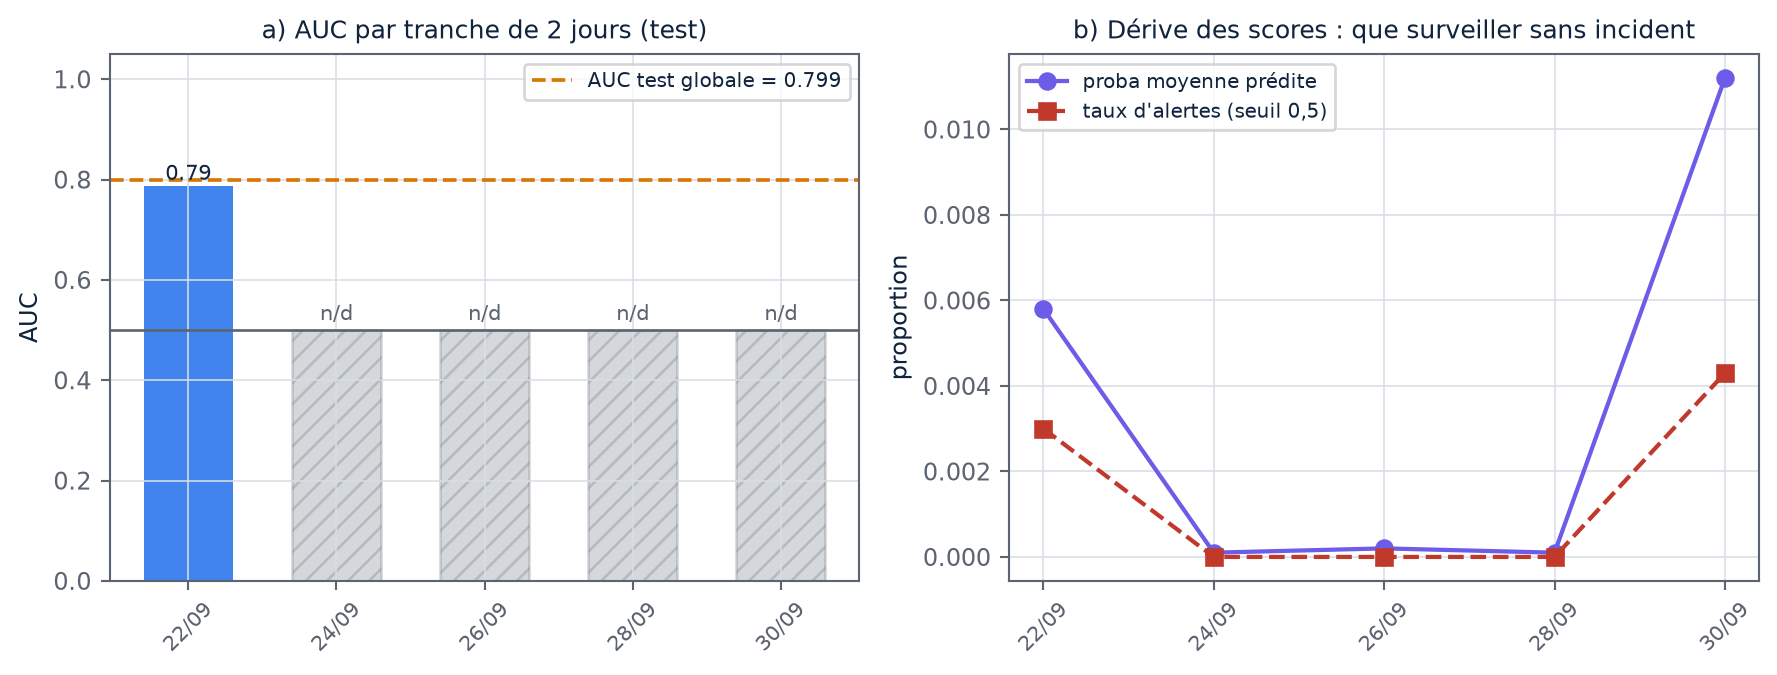
\includegraphics[width=0.80\textwidth]{f33_auc_tranches.png}
\end{center}
\begin{kbox}[Ce que la figure montre (pipeline réel, graine 5534)]
\textbf{a)} L'AUC ne se calcule que sur la tranche du 22/09 (l'incident du
test est concentré là) : \textbf{0,79}, contre \textbf{0,80} sur le test
complet. \textbf{b)} Sans incident, on surveille la \textbf{distribution des
scores} : la proba moyenne remonte de 0,0001 à \textbf{0,0112} et le taux
d'alertes passe à \textbf{0,43 \%} sur la dernière tranche --- signal de
dérive à investiguer avant qu'un incident n'arrive.
\end{kbox}
\end{frame}

\begin{frame}{Le registre de modèles}
\begin{columns}[t]
\begin{column}{0.5\textwidth}
\begin{block}{Ce qu'un registre stocke pour chaque version}
\begin{itemize}
\item Le \textbf{fichier du modèle} (notre \file{.joblib}, 1,1 Mo) et son
empreinte (hash).
\item Les \textbf{données d'entraînement} : fenêtres, colonnes, graine
(\textbf{5534} ici).
\item Les \textbf{métriques de validation} : AUC test 0,80, latence, seuil.
\item Le \textbf{statut} : expérimental, validé, en production, archivé.
\end{itemize}
\end{block}
\end{column}
\begin{column}{0.46\textwidth}
\begin{ebox}[Outils réels]
MLflow, DVC, ou --- suffisant à notre échelle --- un répertoire Git avec un
fichier \file{manifeste.yaml} par version. Le registre répond à une seule
question : \textbf{« quel modèle exactement tournait le 5/10 à 3 h ? »}
\end{ebox}
\begin{wbox}[Lien avec la séance 5]
Le jour de l'intrusion, le registre permet de rejouer les prédictions de la
version en service et de prouver ce que le modèle \textbf{voyait} à ce
moment-là. Sans registre : impossible.
\end{wbox}
\end{column}
\end{columns}
\end{frame}

\begin{frame}[fragile]{Conteneuriser le modèle : Docker en 10 lignes de concept}
\small
\begin{codebox}[L'image = modèle + code de scoring + dépendances figées]
\begin{lstlisting}
FROM python:3.11-slim                    # base figee
WORKDIR /app
COPY nosys_forest.joblib .               # le modele (1,1 Mo)
COPY scorer.py .                         # code de scoring
RUN pip install --no-cache-dir pandas scikit-learn joblib
CMD ["python", "scorer.py"]              # le service
\end{lstlisting}
\end{codebox}
\begin{columns}[t]
\begin{column}{0.48\textwidth}
\begin{kbox}[Pourquoi conteneuriser]
La même image tourne partout : \textbf{mêmes versions} de pandas et
scikit-learn, donc \textbf{mêmes prédictions}. Un modèle qui change de
comportement après une mise à jour de bibliothèque est un incident en
puissance.
\end{kbox}
\end{column}
\begin{column}{0.48\textwidth}
\begin{wbox}[Piège classique]
L'image contient le modèle \textbf{figé au build}. Une nouvelle version du
modèle = une nouvelle image, versionnée et testée --- jamais un écrasement
du fichier en place. C'est le rollback du B3.
\end{wbox}
\end{column}
\end{columns}
\end{frame}

\begin{frame}{Monitoring : que surveiller en production ?}
\begin{center}\footnotesize
\begin{tabular}{@{}p{3.6cm}p{4.4cm}p{4.2cm}@{}}
\toprule
\textbf{Famille} & \textbf{Métrique} & \textbf{Alarme typique}\\
\midrule
Qualité du modèle & AUC recalculée quand la vérité terrain arrive &
AUC $<$ 0,70 pendant 48 h\\
\addlinespace[1pt]
Comportement & taux d'alertes par jour, précision des alertes &
$>$ 3 $\times$ la médiane des 30 derniers jours\\
\addlinespace[1pt]
Santé du service & latence de scoring (moyenne + p99) & p99 $>$ 2 $\times$
la moyenne\\
\addlinespace[1pt]
Entrées & distribution des variables (moyenne, quantiles) & dérive de
\py{cpu\_moy} hors bornes historiques\\
\bottomrule
\end{tabular}
\end{center}
\vspace{1mm}
\begin{kbox}[La règle des deux horloges]
Le monitoring du \textbf{modèle} (AUC, dérive) tourne à l'échelle des
jours ; le monitoring du \textbf{service} (latence, erreurs) tourne à
l'échelle des minutes. Confondre les deux, c'est découvrir un service tombé
une semaine plus tard --- ou alarmer un ingénieur pour une variation de 0,001
d'AUC.
\end{kbox}
\end{frame}

\begin{frame}{Quiz 1 --- MLOps (5 min)}
\begin{qbox}[3 questions]
\begin{enumerate}
\item Le retraining « sur incident majeur » se déclenche quand :\\
(a) une alerte est émise \quad (b) un événement change le régime du système
(migration, nouveau serveur) \quad (c) l'AUC baisse de 0,001
\item Sur les tranches de test sans incident, l'AUC :\\
(a) vaut 0 \quad (b) n'est pas calculable --- on surveille la distribution
des scores \quad (c) vaut 1
\item La version du modèle en production le jour d'un incident se retrouve
grâce à :\\
(a) la mémoire de l'équipe \quad (b) le registre de modèles \quad (c) la
date du fichier
\end{enumerate}
\end{qbox}
\vspace{1mm}
\begin{solbox}[Réponses]
\textbf{1 : b} \quad \textbf{2 : b} --- sans positif, pas d'AUC ; d'où le
suivi de la distribution des scores \quad \textbf{3 : b}
\end{solbox}
\end{frame}
